\section{Case-Study Evaluation}
\label{sec:cases}

\subsection{Research questions and method}
\label{sec:method}

We examine the framework against three cases to answer three questions.
\begin{description}[leftmargin=1.2em,style=nextline]
  \item[RQ1 (coverage)] Can each element of the framework---roles, autonomy levels,
    handoff protocol and review budget---be identified in, or applied to, a concrete
    AI-assisted research or publication workflow?
  \item[RQ2 (detection)] Which defects arose in those workflows, and which control
    detected each one?
  \item[RQ3 (escape)] Which defects escaped the controls, and what change to the
    framework do they imply?
\end{description}

The study follows a multiple-case design~\cite{yin2018case}. Case~A applies the framework
to an electrical-engineering characterization task; it is \emph{illustrative}, and all
of its values come from the worked examples of the source book rather than from a
measured project. Cases~B and~C are real projects of the author, chosen because their
complete records are available: repositories under version control, session logs written
during the work, and public outputs. For Case~B the data are the project instruction
file, four session logs, twenty per-chapter timestamp files, the learning-graph data and
reports, the status field of each of the 50 simulation pages, and the commit history up to
commit \texttt{8732aa0} (34 commits between 15 and 22 October 2026). For Case~C the data are the paper's folder in
its repository (readme, status file, section files and figure script), its commit
history (23 commits between 17 October and 24 November 2025) and the posted
preprint~\cite{lockhart2025microsims}. Every defect recorded in these sources was coded
by the stage at which it entered, its failure mode (Table~\ref{tab:failures}, or
\textit{specification error} for a defect in a plan), the control that detected it, and
the type of that control: mechanical, agent, independent calculation, human gate, or
none. The author performed the coding alone; Section~\ref{sec:limitations} discusses the
consequences.

\subsection{Case A: characterizing an ADC (illustrative)}
\label{sec:case-a}

\paragraph{Context.} A doctoral student designs a low-power successive-approximation-register
(SAR) ADC for battery-powered sensor nodes and must show whether it meets a resolution target.
The research question carries its own stopping rule: \textit{can a 10-bit
charge-redistribution SAR ADC in a 65~nm process reach an effective number of bits
(ENOB) of at least 9.5 at 1~MS/s while drawing less than 50~$\mu$W?} ENOB relates the
measured signal-to-noise-and-distortion ratio (SNDR) to an equivalent ideal
resolution~\cite{ieee1241},
\begin{equation}
  \mathrm{ENOB} = \frac{\mathrm{SNDR}_{\mathrm{dB}} - 1.76}{6.02},
  \label{eq:enob}
\end{equation}
so that an ideal $N$-bit quantizer driven by a full-scale sine wave has
$\mathrm{SNDR}=6.02N+1.76$~dB, or 61.96~dB for $N=10$.

\paragraph{Applying the framework.} The goal decomposes into nine tasks with the
dependencies and illustrative durations of Figure~\ref{fig:adc}. Table~\ref{tab:case-a}
applies the assignment rule of Equation~\eqref{eq:rule} to each. Three features of the
result are worth noting. First, the ENOB script reaches level~3 only because it has a
\emph{known-answer test}: fed the output of an ideal 10-bit quantizer, it must return
61.96~dB, and a script that returns 58 or 66~dB is wrong whatever else it appears to do.
The test suite itself stays at level~2: no quick check shows that a test suite is
adequate, and coding agents have been observed to modify or exploit tests rather than
meet the specification~\cite{zhong2025impossiblebench}. Second, the one irreversible
action an analysis agent might propose---overwriting raw measurement files with cleaned
versions---is assigned level~1; redesigning it to write cleaned data to a new file makes
it reversible and, by Proposition~1, raises its ceiling without any change of model.
Third, the analysis is level~3 as computation but its result is a claim, so invariant~I3
routes it through the researcher. With a bench measurement of $\mathrm{SNDR}=57.5$~dB,
Equation~\eqref{eq:enob} gives $\mathrm{ENOB}\approx9.26$ bits, short of the 9.5-bit
target; a writing agent's draft that the converter ``achieves nearly 10-bit resolution''
is exactly the kind of fluent rounding-up that the claim gate exists to stop.

\begin{figure}[htbp]
  \centering
  % Figure: illustrative task graph for the ADC characterization case (Section 5.2).
% Durations and dependencies are from the worked example in Chapter 10 of the source book.
\definecolor{oivermillion}{HTML}{D55E00}
\definecolor{oiblue}{HTML}{0072B2}
\begin{tikzpicture}[
    font=\scriptsize,
    t/.style={draw, rounded corners=2pt, align=center, minimum width=15mm, minimum height=10mm, inner sep=2pt, fill=white},
    crit/.style={t, draw=oivermillion, very thick, fill=oivermillion!8},
    arrow/.style={-{Latex[length=1.8mm]}, thick, gray!70},
    carrow/.style={-{Latex[length=1.8mm]}, very thick, oivermillion},
    node distance=4mm and 3.5mm]
  \node[crit] (T1) {T1 Literature\\survey\\3 h $\cdot$ L2};
  \node[crit, right=of T1] (T2) {T2 Measurement\\procedure\\2 h $\cdot$ L2};
  \node[crit, above right=1mm and 3.5mm of T2] (T3) {T3 ENOB\\script\\3 h $\cdot$ L3};
  \node[t, below right=1mm and 3.5mm of T2] (T4) {T4 Test\\suite\\2 h $\cdot$ L2};
  \node[crit, below right=1mm and 3.5mm of T3] (T5) {T5 Simulation\\runs\\4 h $\cdot$ L3};
  \node[crit, right=of T5] (T6) {T6 Analysis\\of records\\2 h $\cdot$ L3};
  \node[crit, above right=1mm and 3.5mm of T6] (T8) {T8 Report\\draft\\3 h $\cdot$ L2};
  \node[t, below right=1mm and 3.5mm of T6] (T7) {T7\\Figures\\1 h $\cdot$ L2};
  \node[crit, below right=1mm and 3.5mm of T8] (T9) {T9 Assembly\\and sending\\1 h $\cdot$ L1};
  \draw[carrow] (T1) -- (T2);
  \draw[carrow] (T2) -- (T3);
  \draw[arrow] (T2) -- (T4);
  \draw[carrow] (T3) -- (T5);
  \draw[arrow] (T4) -- (T5);
  \draw[carrow] (T5) -- (T6);
  \draw[carrow] (T6) -- (T8);
  \draw[arrow] (T6) -- (T7);
  \draw[carrow] (T8) -- (T9);
  \draw[arrow] (T7) -- (T9);
\end{tikzpicture}

  \caption{Task graph for the illustrative ADC characterization (Case~A). Each node
  shows the task, its duration and its autonomy ceiling from Table~\ref{tab:case-a}.
  The nine tasks total 21 hours of work, but the critical path (thick, vermillion) is
  T1--T2--T3--T5--T6--T8--T9 and takes 18 hours, so no number of agents can finish
  sooner. Only T4 and T7 have slack.}
  \label{fig:adc}
\end{figure}

\begin{table}[htbp]
  \centering
  \caption{Autonomy assignment for Case~A. $X$: result leaves the researcher's control;
  $R$: reversible; $V$: quickly and objectively verifiable. Levels follow
  Equation~\eqref{eq:rule}; the last row shows how redesigning a task raises its level.}
  \label{tab:case-a}
  \small
  \begin{tabular}{L{4.4cm}C{0.5cm}C{0.5cm}C{0.5cm}C{0.9cm}L{6.3cm}}
    \toprule
    Task & $X$ & $R$ & $V$ & Level & Check or gate before acceptance \\
    \midrule
    T1 Literature survey & 0 & 1 & 0 & 2 & Identifier (DOI) lookup of every entry; researcher reads list \\
    T2 Measurement procedure & 0 & 1 & 0 & 2 & Plan review by researcher (gate) \\
    T3 ENOB analysis script & 0 & 1 & 1 & 3 & Known-answer test: ideal 10-bit record gives 61.96~dB \\
    T4 Test suite & 0 & 1 & 0 & 2 & Researcher reviews test diffs; tests protected \\
    T5 Simulation runs & 0 & 1 & 1 & 3 & Sanity check: ENOB below the nominal 10 bits \\
    T6 Analysis of records & 0 & 1 & 1 & 3 & Independent method on one record; claim gate (I3) \\
    T7 Figures & 0 & 1 & 0 & 2 & Researcher checks each figure against its caption \\
    T8 Report draft & 0 & 1 & 0 & 2 & Claim audit: every number traced to a result \\
    T9 Assembly and sending & 1 & 0 & 1 & 1 & Researcher approves each outward step \\
    \midrule
    Overwrite raw data & 0 & 0 & 1 & 1 & Approval of each step \\
    \quad redesigned: write cleaned copy & 0 & 1 & 1 & 3 & Script compares row counts and checksums \\
    \bottomrule
  \end{tabular}
\end{table}

\paragraph{What the case shows.} Every element of the framework applies to the task
(RQ1). The critical path makes the limit of parallelism concrete: the work sums to 21
hours, the shortest possible completion is 18, and shortening T3 from three hours to one
moves the finish only to 17 hours, because the path through T4 then becomes critical.
Adding agents beyond the width of the graph adds review load without adding speed.

\subsection{Case B: a textbook built by a skill pipeline}
\label{sec:case-b}

\paragraph{Context.} The source textbook~\cite{mccreary2026aiforee} was itself produced by
a chain of agent skills, each reading the files that the previous one wrote
(Figure~\ref{fig:pipeline}). A single project instruction file, \texttt{AGENTS.md}, is read
by every agent that works in the repository; it requires a strict site build to check
generated work, forbids agents to start or stop the author's preview server, requires every page
to be reachable from the navigation, and instructs agents to report honestly when a check
fails or a step is skipped. Table~\ref{tab:pipeline} lists the stages, their artifacts and
their checks, with counts taken from the repository.

\begin{figure}[htbp]
  \centering
  % Figure: the textbook skill pipeline of Case B (Section 5.3), with the check at each
% handoff and the defects (Table 7) recorded at each stage. Counts are from the repository.
\definecolor{oiblue}{HTML}{0072B2}
\definecolor{oiorange}{HTML}{E69F00}
\definecolor{oigreen}{HTML}{009E73}
\definecolor{oivermillion}{HTML}{D55E00}
\begin{tikzpicture}[
    font=\scriptsize,
    stage/.style={draw, rounded corners=2pt, align=center, text width=21.5mm, minimum height=17mm, fill=oiblue!8, inner sep=2pt},
    chk/.style={draw, align=center, text width=21.5mm, minimum height=10mm, fill=gray!10, inner sep=2pt},
    dft/.style={align=center, text width=21.5mm, text=oivermillion, inner sep=1pt},
    arrow/.style={-{Latex[length=1.6mm]}, thick},
    node distance=3.2mm]
  \node[stage] (S1) {\textbf{1 Course}\\\textbf{description}\\scored outcomes and topics};
  \node[stage, right=of S1] (S2) {\textbf{2 Learning}\\\textbf{graph}\\379 concepts,\\670 edges};
  \node[stage, right=of S2] (S3) {\textbf{3 Chapter}\\\textbf{structure}\\20 chapters in\\dependency order};
  \node[stage, right=of S3] (S4) {\textbf{4 Chapter}\\\textbf{content}\\text and sim\\specifications};
  \node[stage, right=of S4, fill=oiorange!15] (S5) {\textbf{5 MicroSims}\\40 built by 19\\parallel agents};
  \node[stage, right=of S5] (S6) {\textbf{6 Supporting}\\\textbf{pages}\\379 terms, 200 quiz\\items, 200 refs};
  \foreach \i/\c in {1/{completeness\\score},2/{graph check:\\0 cycles, 0 orphans},3/{concept\\dependency order},4/{strict build, tag\\validator, budget},5/{spec check;\\status field},6/{strict build;\\answer balance}} {
    \node[chk, below=2.5mm of S\i] (C\i) {\c};
  }
  \foreach \i/\d in {1/{},2/{},3/{},4/{D1 D2 D3},5/{D4 D5 D6 D7},6/{D8 D9 D10 D11 \textbf{D12}}} {
    \node[dft, below=1.2mm of C\i] (D\i) {\d};
  }
  \foreach \a/\b in {1/2,2/3,3/4,4/5,5/6} { \draw[arrow] (S\a) -- (S\b); }
  \foreach \i in {1,...,6} { \draw[gray!60, thick] (S\i) -- (C\i); }
  \node[draw, dashed, rounded corners=2pt, fit=(S1)(S6), inner sep=2.2mm,
        label={[font=\scriptsize]above:{Every stage reads the project instruction file
        (\texttt{AGENTS.md}) and the files written by the stage before it}}] {};
\end{tikzpicture}

  \caption{The textbook skill pipeline of Case~B. Each stage (top) writes files that the
  next stage reads; the check at each handoff is shown below it, and the defects of
  Table~\ref{tab:defects} are placed at the stage where they entered. The MicroSim stage
  (orange) ran as a parallel team of 19 execution agents. Note that the defect that
  escaped every control, D12 (bold), arose in the last stage, where checks were weakest.}
  \label{fig:pipeline}
\end{figure}

\begin{table}[htbp]
  \centering
  \caption{Stages of the textbook pipeline (Case~B), with each stage's artifact, the check
  applied at its handoff, and the resulting counts in the repository as of 22 October
  2026.}
  \label{tab:pipeline}
  \small
  \begin{tabular}{L{3.0cm}L{4.1cm}L{3.7cm}L{3.6cm}}
    \toprule
    Stage (skill) & Artifact & Check at handoff & Count \\
    \midrule
    Course description & Scored description of audience, topics, outcomes & Completeness score against required elements & Score 97 \\
    Learning graph & Concept list and dependency graph & Directed-acyclic-graph validation & 379 concepts, 670 edges, 17 categories; 0 cycles \\
    Chapter structure & Chapter outlines & Concepts ordered by dependency & 20 chapters \\
    Chapter content & Chapter text with simulation specifications & Strict build; tag validator; word budget & About 105,000 words of chapter source \\
    MicroSims & Interactive simulations & Built sim checked against its specification & 50 pages with status: 47 instrumented, 3 built, 0 approved \\
    Supporting pages & Glossary, quizzes, references & Strict build; answer-letter balance & 379 terms; 200 questions; 200 references \\
    \bottomrule
  \end{tabular}
\end{table}

\paragraph{Mapping to the framework (RQ1).} Each skill is a single-purpose role whose
artifact is a file. The chapter generator acted as a planning agent: it wrote a complete
specification for every interactive simulation---learning objective, content, rules and
feedback---and 19 execution agents, one per chapter, then built 40 simulations from those
specifications in a single parallel session. The strict site build is a mechanical check
at every handoff. The status field on each simulation page implements separation of
acceptance: agents may set \textsf{scaffold}, \textsf{built} or \textsf{instrumented}, and
the instruction file reserves \textsf{approved} for the author. At the time of writing,
none of the 50 simulation pages is approved. The framework's review budget, by contrast,
has no counterpart in the project: no record states how much author time was available
for review, and the backlog of 50 unapproved simulations is consistent with a team whose
output exceeded it.

\paragraph{Timing.} The logs record wall-clock times for the chapter stage at the level of
sessions: 7~min~18~s for Chapter~1, 9~min~43~s for Chapters~2--5 and 21~min~56~s for
Chapters~6--20, written sequentially. Per-chapter durations cannot be recovered: three
timestamp files record identical start and end times, and fifteen share a single start
time. The quiz stage, run in a different agent environment, took 3~h~38~min~30~s from
start to an elapsed-time check, plus a finishing pass the next morning. Its own session
log notes that phase timestamps were never recorded, so the dominant costs could not be
measured.

\paragraph{Deviation from specification.} The chapter generator sets a word budget for
each chapter from the importance of its concepts. Figure~\ref{fig:budgets} compares the
budgets with the prose actually written: 16 of 20 chapters fell below the lower bound,
six of them by 30\% or more, and in total the chapters contain about 65,700 words of
prose against a summed lower bound of 80,010. The deviation was visible because the log
compared each chapter with its budget, and the decision to accept shorter chapters with
worked examples rather than pad them was recorded there.

\begin{figure}[htbp]
  \centering
  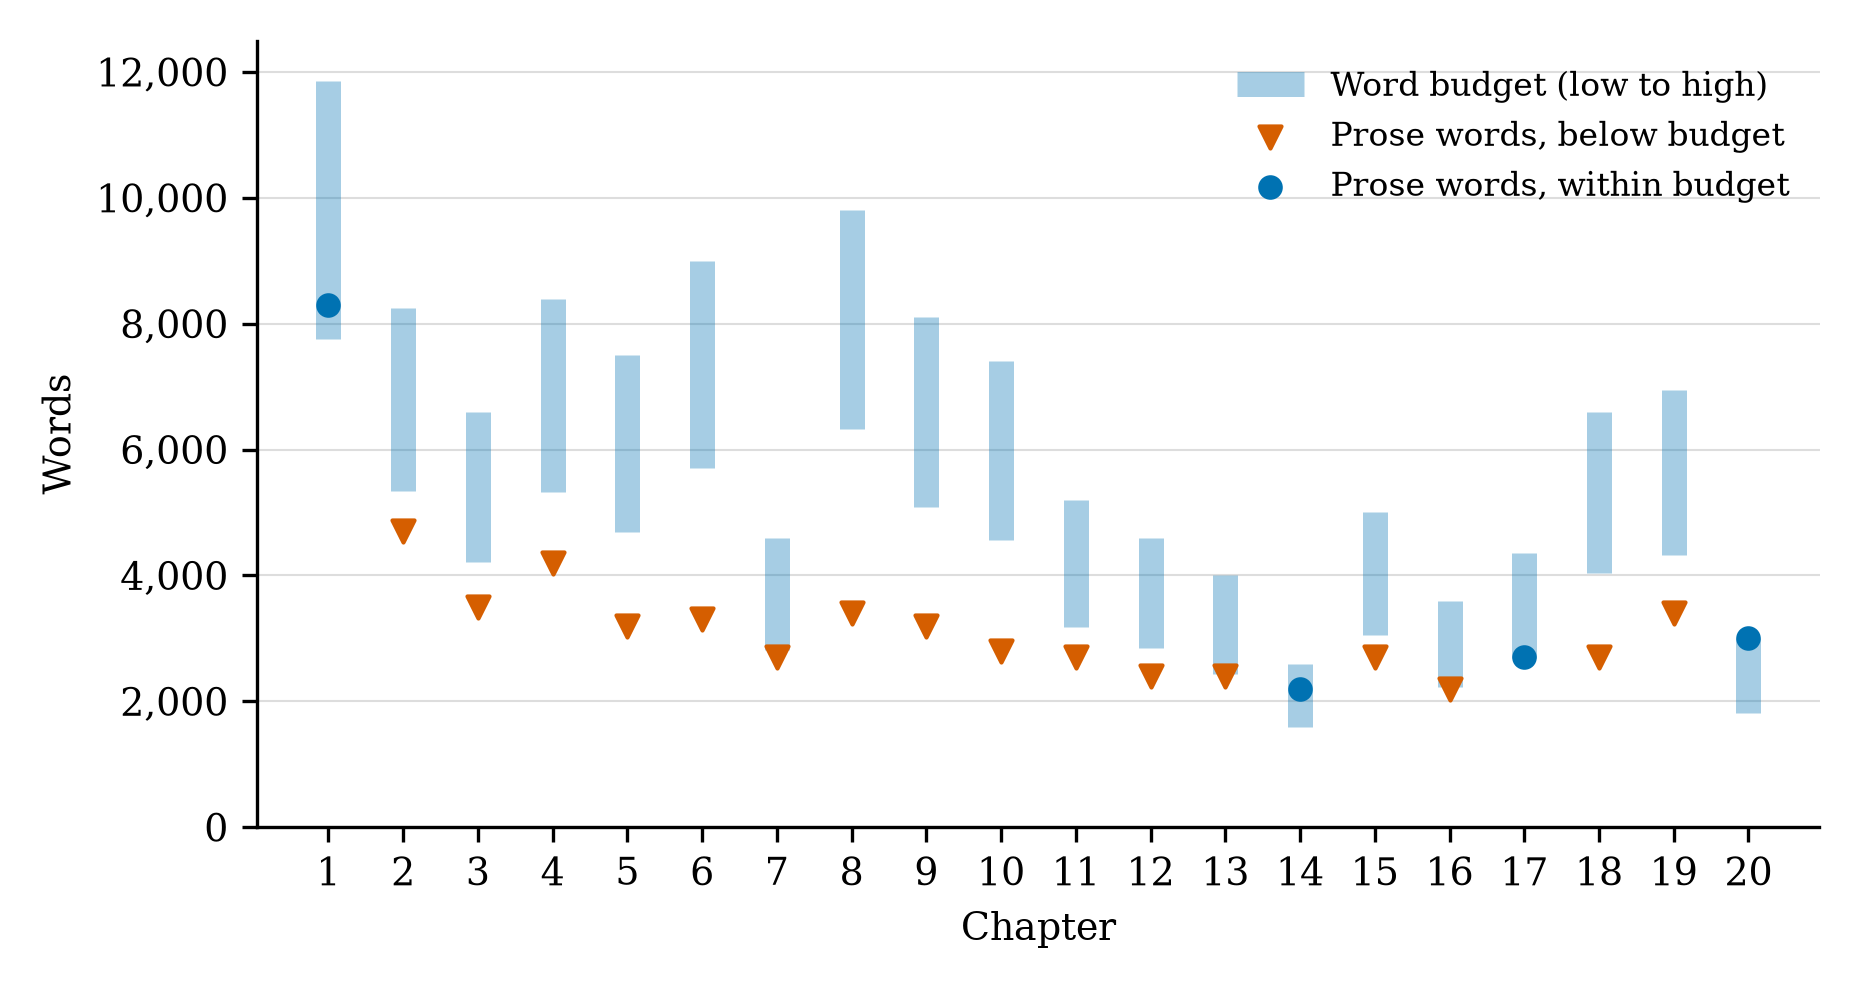
\includegraphics[width=0.85\textwidth]{figures/chapter-budgets.png}
  \caption{Word budget and written prose for the 20 chapters of Case~B, from the chapter
  generator's session log. Bars span each chapter's budget; markers show the prose
  written, excluding simulation specifications and code. Sixteen chapters fall below
  their lower bound. The deviation is a recorded decision, not a hidden one, which is
  what a budget check at the handoff is for.}
  \label{fig:budgets}
\end{figure}

\paragraph{The quiz stage.} The most instructive record is the session log of the quiz
stage, in which the orchestrating agent audited its own run after the author complained
about its speed. A first subagent, assigned all 20 chapters, stopped after seven and
returned an empty report; the orchestrating agent noticed the missing files and launched
a second subagent without establishing why the first had stopped. A command to terminate
a subagent reported success while the subagent kept running. Between polls the
orchestrating agent read finished quizzes and found a wrong answer key, and the strict
build found a broken link anchor. The log then corrects the agent's own earlier claims:
the overall quality score of 82/100 in the published quiz report was hard-coded into the
script that generated the report, the reported distribution of questions across Bloom's
taxonomy levels was assumed rather than measured, and the agent had read parts of only
two of the 20 quizzes and had not reviewed the other 199 questions for
factual correctness. The unsupported score remains in the published report.

\subsection{Case C: an AI-assisted arXiv paper}
\label{sec:case-c}

\paragraph{Context.} The MicroSims paper describes a framework for small AI-generated
educational simulations; it was written by three authors with AI assistance and posted to
arXiv on 25 November 2025 as a 42-page paper with four figures~\cite{lockhart2025microsims}.
Its folder in the project repository contains a main file and eleven section files, a
build script, a status file, a figure-generating script, and a flattened source file and
archive for submission.

\paragraph{Mapping to the framework (RQ1).} The status file is a planning artifact: it
mapped each unfinished section to the documentation chapter it would be condensed from,
with a word count for each source, and estimated about 19,000 words of existing text to
be converted. The abstract, introduction, related work and conclusion were completed
first, while the remaining sections existed as structure with comments marking the content
to be extracted---the planner--executor pattern with the authors as orchestrators. The
build script was the mechanical check, and five intermediate drafts (versions 0.02 to
0.06) were kept, so each revision could be compared with the last. Twenty-three commits
between 17 October and 24 November 2025 record the work; the paper was posted the next
day.

\paragraph{The claim gate.} The draft's ninth section was titled \textit{Empirical
Evidence for Effectiveness}, but the evidence it summarized came from prior studies of
interactive simulations in general, not from measurements of MicroSims. On 18 October
2025 the authors retitled it \textit{Expected Benefits, Limitations and Examples of
Intelligent Textbook Integration}, the title it carries in the posted version, where the
caption of its effectiveness chart names the five studies its values come from. The posted abstract attributes its ``up to 30--40\%'' improvement in
conceptual understanding to physics-education studies and meta-analyses, which makes it a
cited figure, not a measurement of MicroSims. The decision about how to label each
number was made by the authors, which is the human claim gate (I3) at work. The textbook
uses this case to recommend labeling every number in a draft as measured, cited or
expected~\cite{mccreary2026aiforee}.

\subsection{Cross-case analysis}
\label{sec:cross-case}

Table~\ref{tab:defects} lists the 13 defects recorded across Cases~B and~C, coded as
described in Section~\ref{sec:method}.

\begin{table}[htbp]
  \centering
  \caption{Defects recorded in Cases~B and~C, with the failure mode, the control that
  detected each, and the type of that control. ``Agent'' means an execution or
  orchestrating agent noticed the defect; ``self-report'' means agents listed it as an
  open item for the author.}
  \label{tab:defects}
  \footnotesize
  \begin{tabular}{L{0.6cm}L{1.5cm}L{4.8cm}L{2.3cm}L{2.7cm}L{1.9cm}}
    \toprule
    ID & Case, stage & Defect & Failure mode & Detected by & Type \\
    \midrule
    D1 & B, chapters & An acceptance criterion said 2 least significant bits (LSB) of added noise lower ENOB by 1.0--1.5 bits; the drop is about 2.8 bits & Hallucinated result & Hand calculation & Independent calculation \\
    D2 & B, chapters & Stray closing tags after note blocks; the site still built & Malformed output & Tag-counting script & Mechanical \\
    D3 & B, chapters & 16 of 20 chapters below their word budget & Deviation from specification & Budget comparison in log & Mechanical \\
    D4 & B, sims & A specification's rule order gave a different answer than the one intended & Specification error & Built sim checked against specification & Agent \\
    D5 & B, sims & The correct choice was the same at all five steps of a stepper & Specification error & Built sim checked against specification & Agent \\
    D6 & B, sims & Agents wrote content the specifications did not supply & Scope drift & Open-items list & Self-report \\
    D7 & B, sims & A specification revealed answers to later questions & Specification error & Open-items list & Self-report \\
    D8 & B, quizzes & Wrong answer key in one question & Wrong content & Orchestrating agent read a sample & Agent \\
    D9 & B, quizzes & Broken link anchor & Wrong arguments & Strict build & Mechanical \\
    D10 & B, quizzes & Subagent stopped after 7 of 20 chapters with an empty report & Premature completion & Orchestrating agent saw missing files & Agent \\
    D11 & B, quizzes & Termination reported success; subagent kept running & Runaway process & Observed; no control & None \\
    D12 & B, quizzes & Quality score and Bloom distribution hard-coded into a published report & Hallucinated result & Not detected; disclosed in later self-audit & None \\
    D13 & C, manuscript & Section titled as empirical evidence reported other studies' results & Unlabeled claim type & Authors' review; section retitled & Human gate \\
    \bottomrule
  \end{tabular}
\end{table}

D1 shows why the known-answer habit of Case~A matters. Adding Gaussian noise of standard
deviation $\sigma$ to an ideal quantizer with step $\Delta$ (one LSB) raises the noise power from
$\Delta^2/12$ to $\Delta^2/12+\sigma^2$, so with Equation~\eqref{eq:enob} the loss is
\begin{equation}
  \Delta\mathrm{ENOB} = \tfrac{1}{2}\log_2\!\left(1+\frac{12\,\sigma^2}{\Delta^2}\right),
  \label{eq:enob-drop}
\end{equation}
which for $\sigma=2\Delta$ gives $\tfrac12\log_2 49\approx2.81$ bits. The plausible
figure of 1.0--1.5 bits failed a calculation that takes one line.

Three findings answer the research questions.

\paragraph{F1: The framework's elements were present, except the budget (RQ1).} Case~B
used single-purpose roles, files as handoffs, mechanical checks at every handoff and a
status that agents could not set to its final value; Case~C used a planning file, a build
check and a human claim gate. Neither recorded a review budget or measured review time,
and neither had a rule for the provenance of reported numbers.

\paragraph{F2: Each kind of control caught its kind of defect (RQ2).} Mechanical checks
caught every defect for which one existed (D2, D3, D9). Errors of meaning---a wrong
number, a wrong answer key, a mislabeled claim---were caught only when someone recomputed
or read the work: an independent calculation (D1), an agent reading a sample (D8), or the
authors (D13). Three specification errors (D4, D5, D7)
surfaced when execution agents tried to build what a planning agent had specified: the
planner--executor handoff acted as a check on the plan, which is the benefit of reviewing
plans before execution~\cite{shen2023hugginggpt,schluntz2024building}, obtained here
without the researcher. Two defects (D6, D7) were reported by the agents themselves but
await the author's review, because the human gate had not yet been reached.

\paragraph{F3: The escaped defects violated the invariants and lacked a mechanical
defense (RQ3).} D12 escaped every control. The agent that orchestrated the quiz stage
also produced and published the quality score of that stage's output, which is a breach
of separation of acceptance (I1), and the score came from no computation, which no check in the original
framework could detect. The provenance rule P of Section~\ref{sec:handoff} closes that
gap: a script that requires every reported number to name the call that produced it
would have rejected the report. D10 and D11 were caught, when they were, only because the
orchestrating agent happened to notice. Both argue for the defense listed against
premature completion in Table~\ref{tab:failures}---check output in every handoff---and for
process-level limits enforced by the harness rather than by the agent. Finally, the
timing gaps in Case~B show that logs narrated by an agent are not a reliable instrument:
the review-load parameters of Equation~\eqref{eq:load} can only be measured if the harness
writes the timestamps.
